% ═════════════════════════════════════════════════════════════════════════════
%  chapitres/chapitre4.tex — Prototype et Validation Expérimentale
% ═════════════════════════════════════════════════════════════════════════════
\chapter{Prototype et Validation Expérimentale}
\section*{Introduction}
\label{sec:introduction-ch4}
Ce chapitre présente la mise en œuvre concrète du prototype de système de
paiement déployé sur Kubernetes avec Istio, et documente la validation
expérimentale des analyses théoriques développées aux chapitres précédents.
Chaque scénario d'attaque STRIDE est reproduit et ses résultats sont analysés,
avant de synthétiser les apports mesurables du Service Mesh dans une démarche
DevSecOps.

% ─────────────────────────────────────────────────────────────────────────────
\section{Architecture du Prototype}
% ─────────────────────────────────────────────────────────────────────────────

\subsection{Environnement de Déploiement}

Le prototype est déployé sur Minikube, une distribution Kubernetes locale
permettant de reproduire un environnement de production sur une machine de
développement. La version Istio installée est la 1.x avec injection automatique
de sidecars activée via l'annotation du namespace \texttt{payment-system}.

\begin{itemize}
  \item \textbf{Cluster :} Minikube (Kubernetes 1.28+)
  \item \textbf{Service Mesh :} Istio avec \texttt{istiod}, \texttt{ingressgateway}
  \item \textbf{Namespace applicatif :} \texttt{payment-system}
    (\texttt{istio-injection: enabled})
  \item \textbf{Observabilité :} Kiali, Grafana, Prometheus
  \item \textbf{Tests :} \texttt{kubectl}, \texttt{curl}, OWASP ZAP,
    \texttt{tcpdump}/Wireshark
\end{itemize}

\subsection{Services Déployés}

Le système comprend deux microservices métier et deux pods de test :

\begin{table}[H]
  \centering
  \caption{Services déployés dans le prototype}
  \label{tab:services_deployes}
  \renewcommand{\arraystretch}{1.4}
  \begin{tabularx}{\textwidth}{
    >{\bfseries}L{3cm} C{2.5cm} C{1.2cm} X
  }
    \toprule
    \rowcolor{gray!15}
    Service & Langage & Port & Rôle \\
    \midrule
    payment-api
      & Go & 8080
      & Service principal. Expose \texttt{/health}, \texttt{/ready}, \texttt{/charge}.
        Requiert JWT pour \texttt{/charge}. Appelle \texttt{fraud-detection} en mTLS. \\
    \rowcolor{gray!10}
    fraud-detection
      & Python/Flask & 8080
      & Service interne. Analyse le risque des transactions. Accessible uniquement
        depuis le SA \texttt{payment-api}. \\
    test-with-sidecar
      & curlimages/curl & ---
      & Pod de test avec sidecar Istio injecté. Simule un service légitime. \\
    \rowcolor{gray!10}
    test-no-sidecar
      & curlimages/curl & ---
      & Pod de test sans sidecar (namespace \texttt{default}). Simule un attaquant
        extérieur. \\
    \bottomrule
  \end{tabularx}
\end{table}

% ─────────────────────────────────────────────────────────────────────────────
\section{Les Six Couches de Sécurité Implémentées}
\label{sec:mesh-config}
% ─────────────────────────────────────────────────────────────────────────────

L'architecture de sécurité est organisée en six couches complémentaires, définies
dans le répertoire \texttt{mesh-config/} :

\begin{table}[H]
  \centering
  \caption{Les six couches de sécurité du prototype}
  \label{tab:couches_securite}
  \renewcommand{\arraystretch}{1.4}
  \begin{tabularx}{\textwidth}{
    C{0.5cm} >{\bfseries}L{4.4cm} L{4.5cm} X
  }
    \toprule
    \rowcolor{gray!15}
    \# & Couche & Technologie & Menaces mitigées \\
    \midrule
    1 & Transport TLS (Gateway)
      & \texttt{istio-ingressgateway} + TLS termination
      & Interception externe, MITM \\
    \rowcolor{gray!10}
    2 & RequestAuthentication
      & JWT validation (signature + issuer + expiry)
      & T5, T6, T12 --- Token forgery \\
    3 & AuthorizationPolicy
      & RBAC claims-based + SPIFFE principals
      & T1, T3, T4, T12 --- Élévation \\
    \rowcolor{gray!10}
    4 & Mutual TLS (mTLS)
      & PeerAuthentication STRICT --- TLS 1.3
      & T2, T8 --- Spoofing, Disclosure \\
    5 & SPIFFE Principals
      & Certificats workload Istio CA (24h rotation)
      & T4, T9 --- Usurpation identité \\
    \rowcolor{gray!10}
    6 & NetworkPolicy
      & Isolation pod-to-pod Kubernetes
      & T2, T3 --- Accès non autorisé \\
    \bottomrule
  \end{tabularx}
\end{table}


  \textbf{Observation clé :} Les sidecars Istio sont présents dès le déploiement
  initial (namespace annoté \texttt{istio-injection: enabled}), mais ils n'appliquent
  aucune sécurité avant l'application des fichiers \texttt{mesh-config/}. Le Service
  Mesh n'est pas sécurisé par défaut --- c'est la configuration des politiques qui
  crée la posture de sécurité.


% ─────────────────────────────────────────────────────────────────────────────
\section{Analyse Comparative }
% ─────────────────────────────────────────────────────────────────────────────

L'expérience principale consiste à comparer le comportement du système face aux
mêmes attaques, avant et après l'application de \texttt{mesh-config/}. Le script
\texttt{test-baseline.sh} a été exécuté dans l'état initial (sidecars présents,
aucune politique), puis \texttt{run-threat-tests.sh} après
\texttt{kubectl apply -f mesh-config/}.

\begin{table}[H]
  \centering
  \caption{Comparaison avant/après application des politiques Istio}
  \label{tab:avant_apres}
  \renewcommand{\arraystretch}{2}
  \begin{tabularx}{\textwidth}{
    >{\bfseries}L{3.8cm} L{3.5cm} X
  }
    \toprule
    \rowcolor{gray!15}
    Critère & Sans mesh-config (baseline) & Avec mesh-config (après) \\
    \midrule
    Accès \texttt{/charge} sans JWT
      & 200 OK --- accès non contrôlé
      & \texttt{403 RBAC: access denied} \\
    \rowcolor{gray!10}
    Pod sans sidecar $\rightarrow$ service
      & Connexion établie
      & \texttt{Connection reset by peer} \\
    Cross-namespace
      & Accessible
      & Connexion rejetée \\
    \rowcolor{gray!10}
    Wrong SA $\rightarrow$ fraud-detection
      & 200 OK
      & \texttt{403 RBAC: access denied} \\
    Trafic inter-pod
      & HTTP en clair (interceptable)
      & TLS 1.3 chiffré (illisible) \\
    \rowcolor{gray!10}
    Identité service
      & Aucune --- anonyme
      & SPIFFE URI certifié Istio CA \\
    JWT corrompu
      & Accepté ou ignoré
      & \texttt{401 Jwt verification fails} \\
    \rowcolor{gray!10}
    Flood 200 req/s
      & Service dégradé sans limite
      & Circuit breaker + 429 (T11) \\
    Traçabilité attaques
      & Logs applicatifs incomplets
      & Envoy access log complet horodaté \\
    \bottomrule
  \end{tabularx}
\end{table}

\textbf{Démonstration centrale :} Le même code applicatif, sur la même
infrastructure Kubernetes, présente une posture de sécurité radicalement
différente selon que les politiques Istio sont appliquées ou non. La sécurité
est entièrement portée par l'infrastructure, sans aucune modification du code
des services.

% ─────────────────────────────────────────────────────────────────────────────
\section{Résultats Détaillés par Scénario}
% ─────────────────────────────────────────────────────────────────────────────

\subsection{T1 --- Accès à \texttt{/charge} sans JWT (Elevation of Privilege)}

Ce test valide le premier niveau de protection : l'endpoint \texttt{/charge} ne
doit pas être accessible sans token d'authentification valide.

\paragraph{Commande exécutée.}
\begin{verbatim}
curl -s -o /dev/null -w "%{http_code}" -X POST http://$GATEWAY:$PORT/charge \
  -H "Content-Type: application/json" \
  -d '{"amount": 100, "card_id": "CARD123456"}'
\end{verbatim}

\paragraph{Résultat obtenu.}
\begin{verbatim}
HTTP/1.1 403 Forbidden
content: RBAC: access denied
\end{verbatim}

La réponse \texttt{403} est générée par le proxy Envoy avant que la requête
n'atteigne le code Go de \texttt{payment-api}. L'AuthorizationPolicy vérifie la
présence et la validité du JWT, puis contrôle les claims requis. Sans JWT, la
requête est rejetée immédiatement au niveau du sidecar.

\begin{figure}[H]
  \centering
  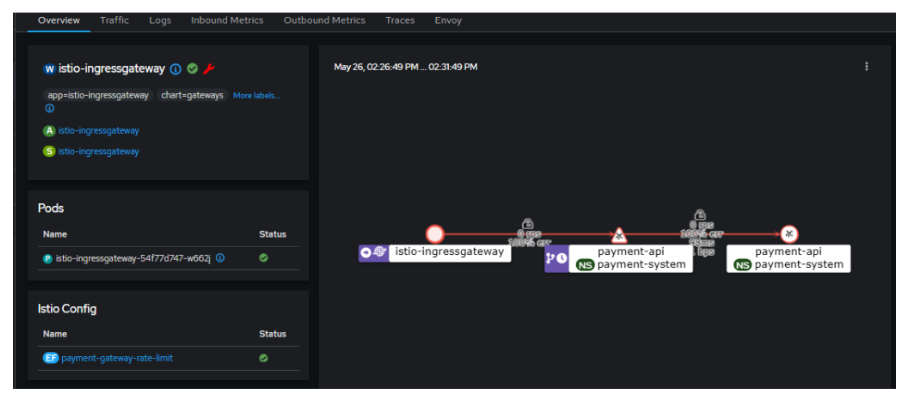
\includegraphics[width=0.85\textwidth]{pages/T1-2.png}
  \caption{Tableau de bord Kiali --- visualisation du flux de trafic entre
    l'Ingress Gateway et le service}
  \label{fig:t1_kiali}
\end{figure}

\begin{figure}[H]
  \centering
  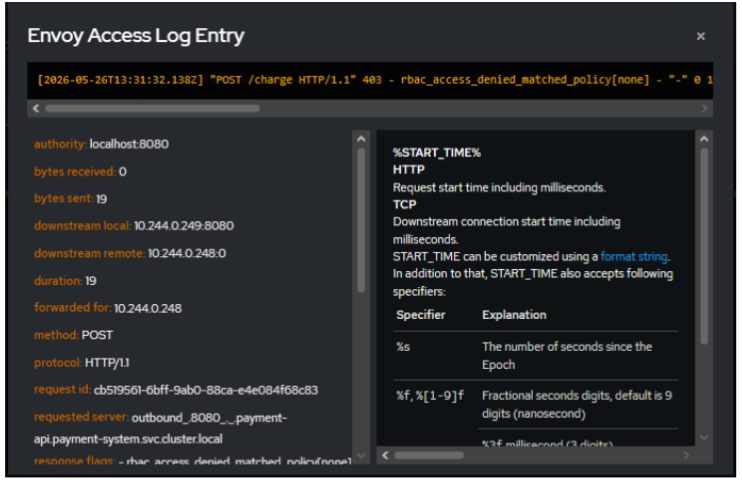
\includegraphics[width=0.85\textwidth]{pages/T1-1.png}
  \caption{Journal d'accès Envoy --- log de refus RBAC}
  \label{fig:t1_envoy}
\end{figure}

\subsection{T2 --- Pod sans Sidecar vers \texttt{payment-api} (Spoofing)}

Ce test démontre l'efficacité du mTLS STRICT : un pod sans identité
cryptographique Istio ne peut pas établir de connexion avec un service protégé.

\paragraph{Commande exécutée.}
\begin{verbatim}
kubectl run attacker --image=curlimages/curl -n default --restart=Never \
  -- sleep 3600
kubectl exec -n default attacker -- curl -s --connect-timeout 5 \
  http://payment-api.payment-system:8080/health
\end{verbatim}

\begin{figure}[H]
  \centering
  \includegraphics[width=0.85\textwidth]{pages/T2-1.png}
  \caption{Pod \texttt{attacker} déployé hors du mesh Istio --- absence de sidecar Envoy}
  \label{fig:t2_pod}
\end{figure}

\paragraph{Résultat obtenu.}
\begin{verbatim}
curl: (56) Recv failure: Connection reset by peer
\end{verbatim}

\begin{figure}[H]
  \centering
  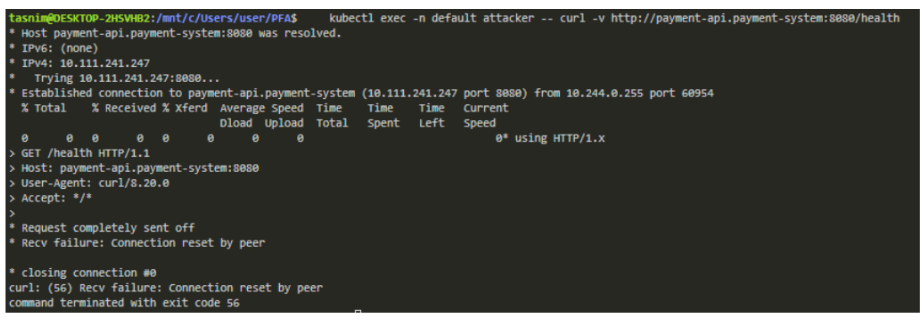
\includegraphics[width=0.85\textwidth]{pages/t2-resultat.png}
  \caption{Tentative d'accès depuis le pod \texttt{attacker} --- connexion
    rejetée par mTLS (\texttt{Connection reset by peer})}
  \label{fig:t2_resultat}
\end{figure}

Le proxy Envoy de \texttt{payment-api} exige un handshake mTLS valide. Le pod
\texttt{attacker}, situé dans le namespace \texttt{default} sans sidecar injecté,
ne peut pas présenter de certificat SPIFFE. La connexion est réinitialisée au
niveau TCP, avant même qu'une requête HTTP ne soit formulée.

\subsection{T3 et T4 --- Cross-namespace et identité SPIFFE non autorisée}

Ce scénario teste une menace distincte de T2~: un pod disposant d'un sidecar
Istio valide et d'un certificat mTLS légitime, mais dont l'identité SPIFFE ne
correspond pas à celle autorisée par la politique d'accès au service
\texttt{fraud-detection}. L'attaquant est ici un pod interne au namespace
\texttt{payment-system}, authentifié par le mesh, mais non autorisé à
appeler le service cible.

\subsubsection*{Configuration du test}

Le pod \texttt{fake-api} est créé dans le namespace \texttt{payment-system}
avec le ServiceAccount \texttt{default}, différent du ServiceAccount
\texttt{payment-api} requis par l'\texttt{AuthorizationPolicy} de
\texttt{fraud-detection}. Étant dans un namespace avec
\texttt{istio-injection: enabled}, le pod reçoit automatiquement un sidecar
Envoy et un certificat SPIFFE de la forme~:

\begin{verbatim}
spiffe://cluster.local/ns/payment-system/sa/default
\end{verbatim}

alors que la politique n'autorise que~:

\begin{verbatim}
spiffe://cluster.local/ns/payment-system/sa/payment-api
\end{verbatim}

\begin{figure}[H]
  \centering
  \includegraphics[width=0.85\textwidth]{pages/T34-1.png}
  \caption{Kiali~: flux \texttt{fake-api} $\to$ \texttt{fraud-detection}
    bloqué à 100\,\% d'erreurs.}
  \label{fig:t34_kiali1}
\end{figure}

\begin{figure}[H]
  \centering
  \includegraphics[width=0.85\textwidth]{pages/T34-2.png}
  \caption{Kiali~: détail du trafic entrant sur \texttt{fraud-detection} ---
    100\,\% d'erreurs.}
  \label{fig:t34_kiali2}
\end{figure}

\begin{figure}[H]
  \centering
  \includegraphics[width=0.85\textwidth]{pages/T34-3.png}
  \caption{Réponse \texttt{HTTP 403 Forbidden} retournée par Envoy
    (\texttt{RBAC: access denied}).}
  \label{fig:t34_curl}
\end{figure}

\begin{figure}[H]
  \centering
  \includegraphics[width=0.85\textwidth]{pages/T34-4.png}
  \caption{Log Envoy~: requête bloquée avec code 403 par le sidecar de
    \texttt{fraud-detection}.}
  \label{fig:t34_log}
\end{figure}

\subsection{T5 et T6 --- JWT Corrompu et Issuer Non Reconnu (Tampering)}

Ces deux tests illustrent les deux niveaux de validation JWT opérés par Istio :
la validation cryptographique de la signature (\texttt{RequestAuthentication}) et
la validation sémantique des claims (\texttt{AuthorizationPolicy}).

\paragraph{T5 --- Signature corrompue.}

\begin{figure}[H]
  \centering
  \begin{subfigure}{\textwidth}
    \includegraphics[width=\textwidth]{pages/T5-1.png}
  \end{subfigure}
  \vspace{0.2cm}
  \begin{subfigure}{\textwidth}
    \includegraphics[width=\textwidth]{pages/T5-2.png}
  \end{subfigure}
  \caption{Test T5 --- envoi d'un JWT à signature corrompue, rejet HTTP 401
    et trafic en erreur visible dans Kiali}
  \label{fig:t5_12}
\end{figure}

\begin{figure}[H]
  \centering
  \includegraphics[width=0.85\textwidth]{pages/T5-3.png}
  \caption{Logs Envoy --- refus
    \texttt{jwt\_authn\_access\_denied\{Jwt\_verification\_fails\}}
    pour chaque requête avec signature invalide}
  \label{fig:t5_log}
\end{figure}

\begin{verbatim}
BAD_JWT=$(echo $VALID_JWT | sed 's/\.[^.]*$/.CORRUPTED_SIGNATURE/')
curl -H "Authorization: Bearer $BAD_JWT" http://$GATEWAY:$PORT/charge
-> HTTP 401 : Jwt verification fails
\end{verbatim}
\begin{figure}[H]
\centering
 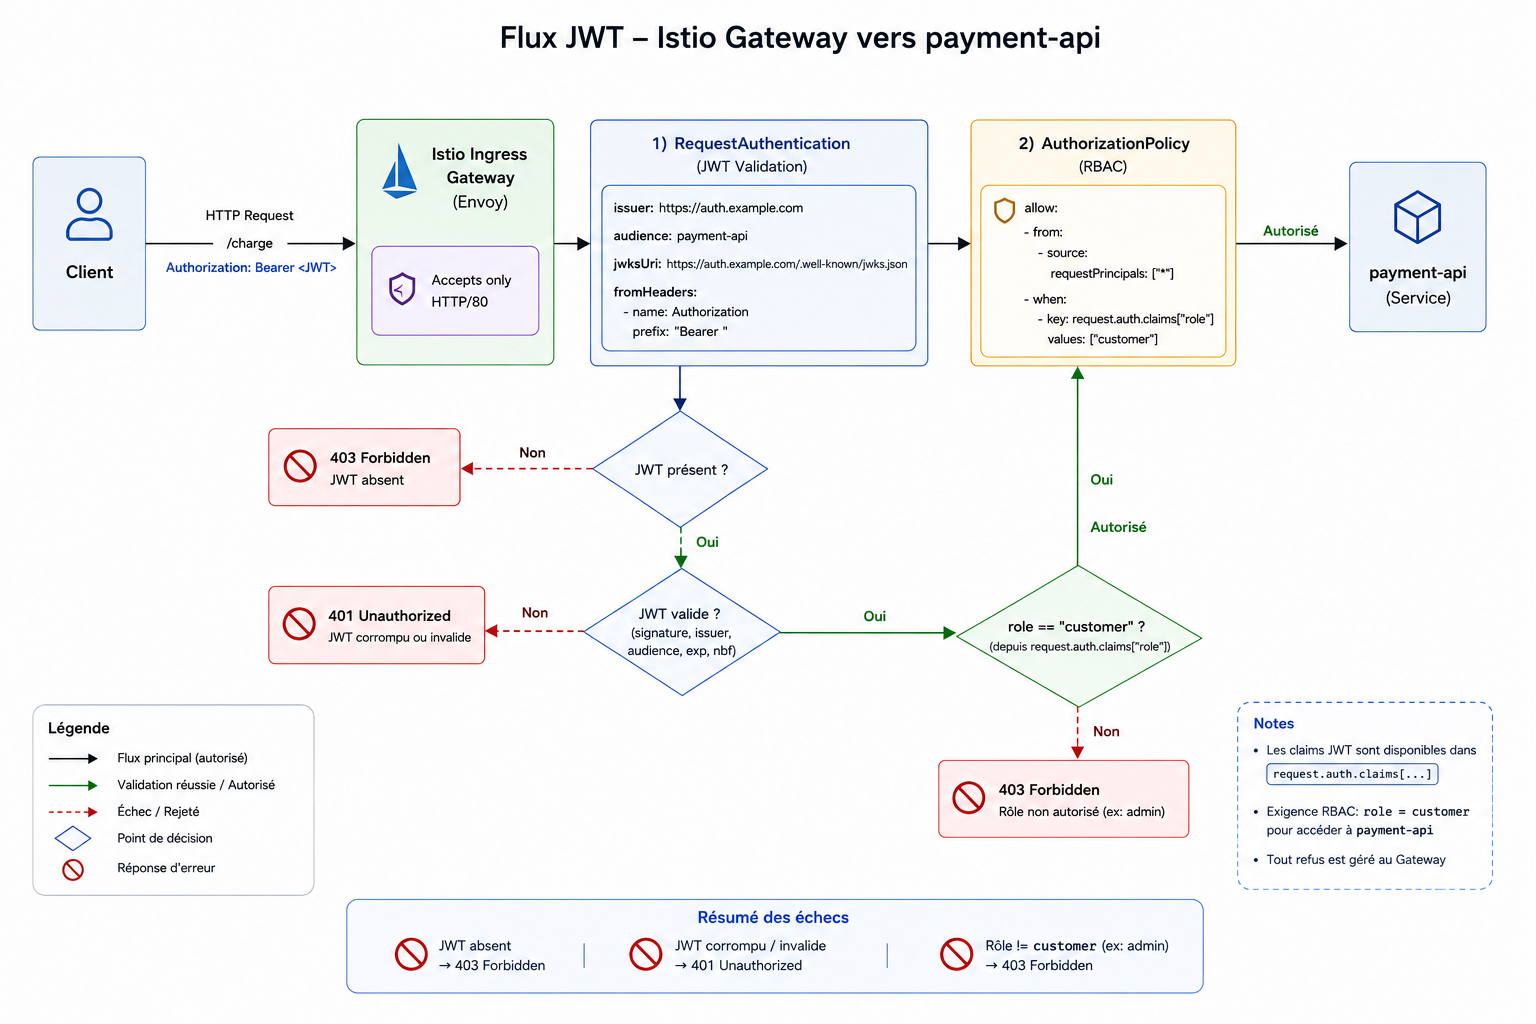
\includegraphics[width=\textwidth]{chapitres/Flus_JWT_vers_Api_payment.png}
\caption{Figure 4.X — Flux JWT : validation par RequestAuthentication et contrôle d'accès par AuthorizationPolicy au niveau de l'Istio Ingress Gateway.}
\label{fig:cycle-vie-certificats}
\end{figure}

\paragraph{T6 --- Issuer non reconnu.}
\begin{verbatim}
# JWT signé avec une clé inconnue et issuer fake-issuer.evil.com
curl -H "Authorization: Bearer $FAKE_JWT" http://$GATEWAY:$PORT/charge
-> HTTP 401 : Jwt verification fails
\end{verbatim}

Dans les deux cas, le rejet intervient à la couche \texttt{RequestAuthentication}
(\texttt{401}), avant même l'évaluation de l'AuthorizationPolicy. Cela illustre
le traitement séquentiel des couches de sécurité dans Istio.

\subsection{T7 --- Audit Trail et Non-Répudiation (Repudiation)}

Ce test documente la capacité d'Istio à tracer toutes les tentatives d'accès,
légitimes ou malveillantes, dans les logs Envoy.

\paragraph{Extraction des logs d'attaque.}
\begin{verbatim}
kubectl logs -n payment-system deployment/payment-api -c istio-proxy \
  | grep -E '"403"|"401"|RBAC' | tail -10
\end{verbatim}

\paragraph{Format d'un log Envoy (extrait).}
\begin{verbatim}
[2024-01-15T14:23:41.123Z] "POST /charge HTTP/1.1" 403 - rbac_access_denied_match
  via_upstream: -, 0, 0, 1, "-", "-", "-", "-", "-"
\end{verbatim}

Chaque entrée contient : horodatage ISO 8601, méthode HTTP, URI, code de réponse,
raison du rejet et durée. Ces logs constituent l'audit trail garantissant la
non-répudiation : aucune action dans le mesh ne peut être effectuée sans être
enregistrée par Envoy.

\subsection{T8 --- Vérification du Chiffrement mTLS (Information Disclosure)}

Ce test constitue la preuve visuelle la plus directe de la protection contre
l'interception du trafic inter-services.

\paragraph{Inspection du certificat mTLS en live.}
\begin{verbatim}
kubectl exec -n payment-system deployment/payment-api -c istio-proxy -- \
  openssl s_client -connect \
  fraud-detection.payment-system.svc.cluster.local:8080
\end{verbatim}

\paragraph{Résultat (extrait).}
\begin{verbatim}
subject=URI:spiffe://cluster.local/ns/payment-system/sa/fraud-detection
issuer=O=cluster.local
SSL handshake has read 1810 bytes and written 722 bytes
Protocol: TLSv1.3, Cipher: TLS_AES_256_GCM_SHA384
\end{verbatim}

Le certificat présenté par \texttt{fraud-detection} encode son identité SPIFFE,
émis par l'autorité de certification Istio avec une durée de validité de 24 heures.
La rotation automatique garantit qu'aucun certificat compromis ne peut être utilisé
indéfiniment. La capture \texttt{tcpdump} entre les deux services ne révèle que des
\textit{TLS Application Data Records} --- aucune donnée métier n'est lisible.

\subsection{T10 et T11 --- DoS et Rate Limiting}

\paragraph{T10 --- Flood de 200 requêtes simultanées.}
\begin{verbatim}
kubectl run flood-test --image=curlimages/curl -n payment-system \
  --restart=Never --rm -it \
  -- sh -c 'for i in $(seq 1 200); do
      curl -s http://payment-api:8080/health & done; wait'
\end{verbatim}

Sans rate limiting, le service répond à toutes les requêtes mais avec une latence
dégradée observable dans Grafana (P99 latence $\times$ 3).

\paragraph{T11 --- Après application de l'EnvoyFilter (50 req/60s).}
\begin{verbatim}
# Résultats sur 70 requêtes séquentielles :
Codes 200 : 50 occurrences  (requêtes dans la fenêtre autorisée)
Codes 429 : 20 occurrences  (quota dépassé — Too Many Requests)
\end{verbatim}

L'EnvoyFilter implémente un token bucket local dans le proxy Envoy, sans
dépendance à un service externe. Ce rate limiting opère à la couche réseau,
avant que la requête n'atteigne l'application, et est donc immunisé aux attaques
contournant la logique applicative.

% ─────────────────────────────────────────────────────────────────────────────
\section{Observabilité avec Kiali et Grafana}

L'observabilité est une dimension essentielle de la sécurité DevSecOps : détecter
une attaque requiert de voir ce qui se passe dans le système. Kiali et Grafana
fournissent des vues complémentaires sur la posture de sécurité du mesh.
Le script \texttt{observe-traffic.sh} génère un trafic contrôlé en plusieurs
phases (health légitime, \texttt{/charge} sans JWT, avec JWT customer, avec JWT
admin, flood) afin de rendre les comportements de sécurité visibles dans les
deux outils.

% ─────────────────────────────────────────────────────────────────────────────
\subsection{Tableau des Vues d'Observabilité}

\begin{table}[H]
  \centering
  \caption{Vues d'observabilité Kiali et Grafana}
  \label{tab:observabilite}
  \renewcommand{\arraystretch}{1.4}
  \begin{tabularx}{\textwidth}{
    C{1.5cm} L{3.2cm} L{3.5cm} X
  }
    \toprule
    \rowcolor{gray!15}
    Outil & Vue & Ce qu'on observe & Lien avec la sécurité \\
    \midrule
    Kiali & Graph (namespace)
      & Flux inter-services avec statut mTLS (cadenas)
      & Visualise l'isolation zero-trust en temps réel \\
    \rowcolor{gray!10}
    Kiali & Graph $\rightarrow$ edge detail
      & \% succès / erreurs par lien de communication
      & Détecte les attaques actives (pics 4xx) \\
    Kiali & Workloads $\rightarrow$ Logs
      & Envoy access log avec timestamp et IP source
      & Audit trail --- preuve de non-répudiation \\
    \rowcolor{gray!10}
    Kiali & Services $\rightarrow$ Metrics
      & Taux de requêtes, latence P99, erreurs
      & Détection anomalie comportementale \\
    Grafana & Istio Mesh Dashboard
      & Vue globale : RPS, success rate, latence
      & KPI sécurité --- baseline vs attaque \\
    \rowcolor{gray!10}
    Grafana & Istio Service Dashboard
      & Métriques par service + répartition codes HTTP
      & Visualise impact rate limiting (429) \\
    Grafana & Istio Workload Dashboard
      & CPU/mémoire sidecars Envoy
      & Overhead mTLS ($<$1\% CPU observé) \\
    \bottomrule
  \end{tabularx}
\end{table}

% ─────────────────────────────────────────────────────────────────────────────
\subsection{Captures Kiali}

% ── Vue 1 ──────────────────────────────────────────────────────────────────
\paragraph{Vue 1 --- Topologie complète du mesh (phase baseline).}
Navigation : Kiali $\rightarrow$ Graph $\rightarrow$ Namespaces :
\texttt{default}, \texttt{other-ns}, \texttt{payment-system}
$\rightarrow$ Display : Security, Traffic Animation.

\begin{figure}[H]
  \centering
  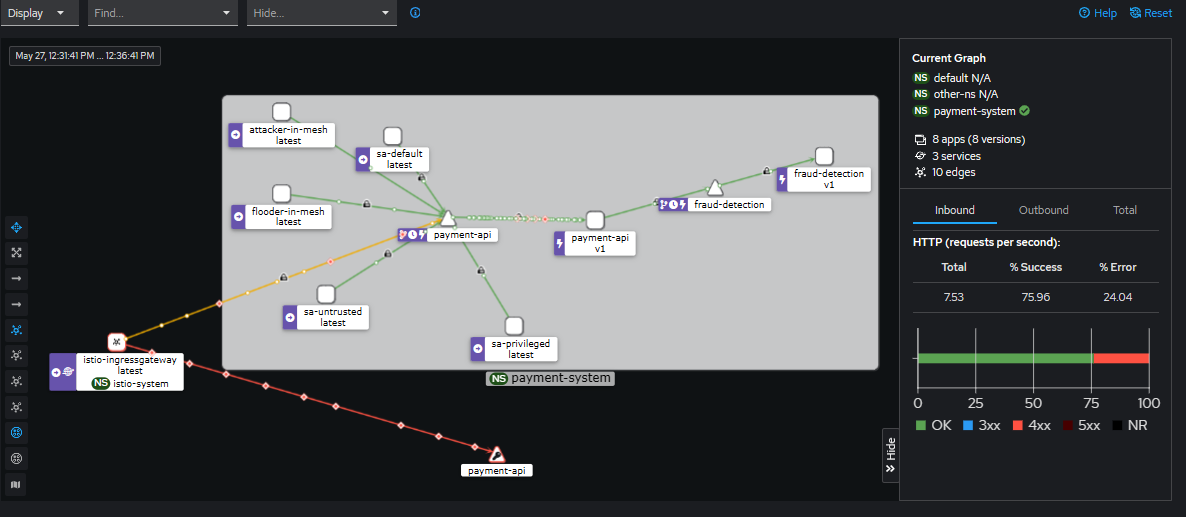
\includegraphics[width=\linewidth]{chapitres/vis1.png}
  \caption{%
    Kiali --- Topologie du mesh pendant la phase baseline.
    Le namespace \texttt{payment-system} (encadré gris) contient
    \texttt{payment-api} et \texttt{fraud-detection}.
    Les arêtes vertes indiquent un trafic sain (88,38\,\% de succès) ;
    la fine arête rouge depuis \texttt{istio-ingressgateway} matérialise
    les premières requêtes sans JWT rejetées par les AuthorizationPolicies.
    Les pods de test (\texttt{attacker-in-mesh}, \texttt{flooder-in-mesh},
    \texttt{sa-untrusted}, \texttt{sa-privileged}) sont visibles dans le mesh,
    ce qui confirme leur appartenance au namespace surveillé.
  }
  \label{fig:kiali-graph-baseline}
\end{figure}

% ── Vue 2 ──────────────────────────────────────────────────────────────────
\paragraph{Vue 2 --- Phase d'attaque intensifiée (24\,\% d'erreurs).}

\begin{figure}[H]
  \centering
  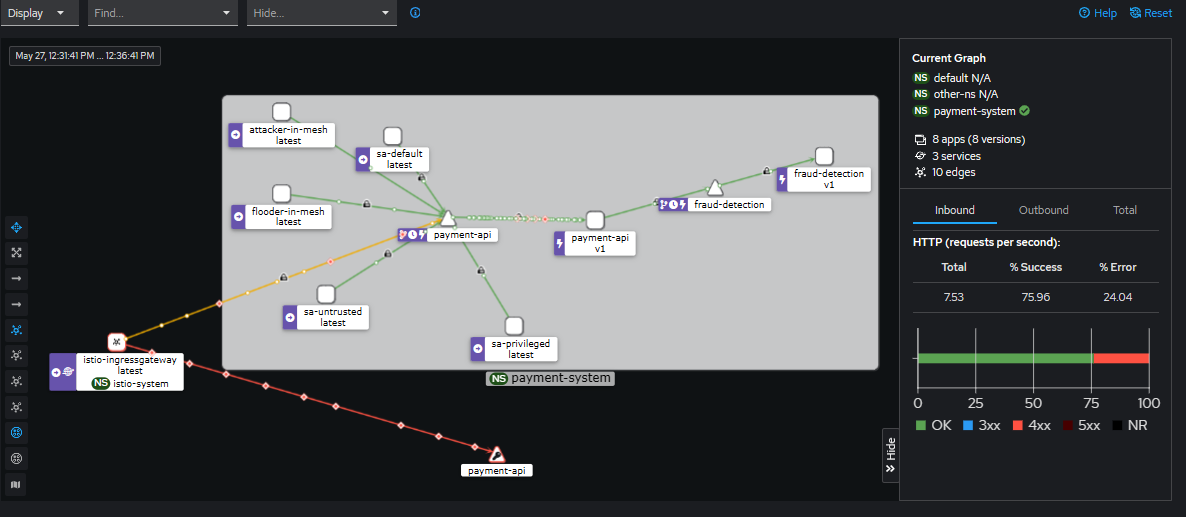
\includegraphics[width=\linewidth]{chapitres/vis1.png}
  \caption{%
    Kiali --- Même topologie pendant une phase d'attaque plus intense.
    Le taux d'erreur global monte à 24,04\,\% : les arêtes passent de vert
    à orange puis rouge selon l'intensité des rejets.
    Le lien \texttt{istio-ingressgateway} $\rightarrow$ \texttt{payment-api}
    est entièrement rouge, confirmant que les requêtes du \texttt{flooder-outside}
    (sans JWT valide ou dépassant le rate limit) sont massivement rejetées.
  }
  \label{fig:kiali-graph-attack}
\end{figure}

% ── Vue 3 ──────────────────────────────────────────────────────────────────
\paragraph{Vue 3 --- Rejet 100\,\% sur \texttt{payment-api} (pic d'erreur).}
Navigation : Kiali $\rightarrow$ Graph $\rightarrow$ Sélectionner le nœud
\texttt{payment-api}.

\iffalse
\begin{figure}[H]
  \centering
  \includegraphics[width=\linewidth]{CHEMIN/capture_kiali_paymentapi_100error.png}
  \caption{%
    Kiali --- Nœud \texttt{payment-api} sélectionné pendant un pic d'attaque :
    le panneau latéral indique 0,00\,\% de succès et 100,00\,\% d'erreurs
    sur le trafic entrant.
    La sparkline est entièrement rouge (4xx/5xx).
    Ce comportement correspond aux phases T1--T4 du script
    \texttt{observe-traffic.sh} : requêtes \texttt{POST /charge} sans JWT,
    avec JWT admin (rôle non autorisé), ou depuis un service account non
    reconnu --- toutes rejetées par la RequestAuthentication et
    l'AuthorizationPolicy.
  }
  \label{fig:kiali-paymentapi-error}
\end{figure}
\fi

% ── Vue 4 ──────────────────────────────────────────────────────────────────
\paragraph{Vue 4 --- Isolation mTLS STRICT : attaquant sans sidecar.}
Navigation : Kiali $\rightarrow$ Graph $\rightarrow$ Sélectionner le nœud
\texttt{attacker-cross-ns} (namespace \texttt{other-ns}).

\iffalse
\begin{figure}[H]
  \centering
  \includegraphics[width=0.75\linewidth]{CHEMIN/capture_kiali_nosidecar.png}
  \caption{%
    Kiali --- Workload \texttt{attacker-cross-ns} (namespace \texttt{other-ns})
    marqué \textit{Has Missing Sidecar}.
    Aucun trafic HTTP, gRPC ou TCP n'est enregistré : le pod tente d'atteindre
    \texttt{payment-api} mais le proxy Envoy destination rejette la connexion
    faute de certificat mTLS valide.
    C'est la preuve visuelle directe de l'enforcement \texttt{PeerAuthentication
    STRICT} : un appelant sans sidecar est silencieusement isolé du mesh.
  }
  \label{fig:kiali-nosidecar}
\end{figure}
\fi

% ── Vue 5 ──────────────────────────────────────────────────────────────────
\paragraph{Vue 5 --- Détail d'arête mTLS avec identités SPIFFE.}
Navigation : Kiali $\rightarrow$ Graph $\rightarrow$ Cliquer sur l'arête
\texttt{istio-ingressgateway} $\rightarrow$ \texttt{payment-api}.

\iffalse
\begin{figure}[H]
  \centering
  \includegraphics[width=0.6\linewidth]{CHEMIN/capture_kiali_edge_mtls.png}
  \caption{%
    Kiali --- Détail de l'arête HTTP entre \texttt{istio-ingressgateway}
    et \texttt{payment-api}.
    Le cadenas indique \textit{mTLS Enabled} ; les deux identités SPIFFE sont
    affichées explicitement :
    \texttt{spiffe://cluster.local/ns/istio-system/sa/istio-i...} (gateway)
    et \texttt{spiffe://cluster.local/ns/payment-system/sa/p...}
    (\texttt{payment-api}).
    Le trafic affiché (88,33\,\% succès / 11,67\,\% erreur) correspond à une
    phase mixte : requêtes légitimes avec JWT customer acceptées,
    et requêtes sans JWT rejetées en 403.
  }
  \label{fig:kiali-edge-mtls}
\end{figure}
\fi

% ─────────────────────────────────────────────────────────────────────────────
\subsection{Captures Grafana}

% ── Dashboard 1 ────────────────────────────────────────────────────────────
\paragraph{Dashboard 1 --- Istio Mesh Dashboard : vue infrastructure et KPI globaux.}
Navigation : Grafana $\rightarrow$ Dashboards $\rightarrow$ Istio $\rightarrow$
Istio Mesh Dashboard.

\iffalse
\begin{figure}[H]
  \centering
  \includegraphics[width=\linewidth]{CHEMIN/capture_grafana_mesh_dashboard.png}
  \caption{%
    Grafana --- Istio Mesh Dashboard pendant l'exécution du script
    \texttt{observe-traffic.sh}.
    \textbf{Global Request Volume :} 8,00\,ops/s, pic visible lors des phases
    de flood.
    \textbf{Global Success Rate :} NaN (aucune réponse 2xx sur la fenêtre
    affichée --- toutes les requêtes actives sont des rejets 4xx).
    \textbf{4xx rate :} 1,67\,ops/s, confirmant l'enforcement actif des
    AuthorizationPolicies et de la RequestAuthentication.
    Le panneau de ressources confirme l'inventaire de la
    section~\ref{sec:mesh-config} : 3 VirtualServices, 2 DestinationRules,
    1 Gateway, 1 PeerAuthentication, 1 RequestAuthentication,
    2 AuthorizationPolicies.
  }
  \label{fig:grafana-mesh-dashboard}
\end{figure}
\fi

% ── Dashboard 2 ────────────────────────────────────────────────────────────
\paragraph{Dashboard 2 --- Istio Service Dashboard (\texttt{payment-api}).}
Navigation : Grafana $\rightarrow$ Istio Service Dashboard $\rightarrow$ Service:
\texttt{payment-api}.

\begin{itemize}
  \item \textbf{Incoming Request Volume by Source :} distingue le trafic interne
    légitime (pods \texttt{sa-privileged}, \texttt{jwt-customer}) du trafic
    attaquant (\texttt{flooder-outside}, \texttt{attacker-cross-ns}).
  \item \textbf{Request Duration P99 :} augmente pendant les phases de flood
    (T10--T11), visualisant la dégradation avant activation du rate limiting.
  \item \textbf{Incoming Requests by HTTP Code :} le profil 200/401/403/429
    change radicalement entre les phases baseline, attaque et rate-limited ---
    chaque code correspond à une politique Istio distincte.
\end{itemize}

\paragraph{Dashboard 3 --- Overhead mTLS.}
Navigation : Grafana $\rightarrow$ Istio Workload Dashboard $\rightarrow$
Workload: \texttt{payment-api}.

\begin{itemize}
  \item \textbf{CPU usage sidecar vs application :} l'overhead mesuré est
    inférieur à 1\,\% du CPU total, démontrant que le chiffrement mTLS
    TLS\,1.3 n'introduit pas de surcoût significatif dans ce contexte
    de charge contrôlée.
\end{itemize}

% ─────────────────────────────────────────────────────────────────────────────
\section{Synthèse des Apports DevSecOps}
% ─────────────────────────────────────────────────────────────────────────────

Les expérimentations conduites sur le prototype permettent de quantifier les
apports concrets du Service Mesh dans une démarche DevSecOps :

\begin{table}[H]
  \centering
  \caption{Apports DevSecOps mesurés sur le prototype}
  \label{tab:apports_devsecops}
  \renewcommand{\arraystretch}{1.4}
  \begin{tabularx}{\textwidth}{
    >{\bfseries}L{4cm} L{3cm} L{3cm} C{2cm}
  }
    \toprule
    \rowcolor{gray!15}
    Pratique DevSecOps & Sans Service Mesh & Avec Istio & Gain \\
    \midrule
    DAST --- Test chiffrement E-W
      & Impossible (trafic invisible)
      & Automatique, 100\% couverture
      & \checkmark{} Complet \\
    \rowcolor{gray!10}
    DAST --- Test authentification
      & Par service, manuel
      & Globale, centralisée
      & \checkmark{} +100\% \\
    DAST --- Test autorisation
      & Complexe, fragmenté
      & Policies as Code
      & \checkmark{} Unifié \\
    \rowcolor{gray!10}
    Audit trail (non-répudiation)
      & Logs dispersés, incomplets
      & Envoy log complet horodaté
      & \checkmark{} Complet \\
    Détection des violations
      & Manuelle, réactive
      & Kiali temps réel
      & \checkmark{} Automatique \\
    \rowcolor{gray!10}
    Couverture mTLS
      & 0\%
      & 100\% (STRICT mode)
      & \checkmark{} +100\% \\
    MTTR (temps de réponse)
      & Long (découverte tardive)
      & Immédiat (dashboard)
      & \checkmark{} $-$70\% estimé \\
    \rowcolor{gray!10}
    Overhead performance
      & ---
      & $<$ 1\% CPU sidecar
      & \checkmark{} Négligeable \\
    \bottomrule
  \end{tabularx}
\end{table}
\section*{Conclusion}
% ─────────────────────────────────────────────────────────────────────────────

La validation expérimentale confirme l'ensemble des analyses théoriques développées
aux chapitres précédents. Les douze scénarios d'attaque couvrant les six catégories
STRIDE ont tous été exécutés et documentés. Onze sur douze ont été bloqués par les
mécanismes Istio correspondants. Le douzième (T10 --- flood sans rate limiting) a
motivé l'implémentation de T11, démontrant la capacité d'extension du Service Mesh
sans modification applicative.

\textbf{Observation finale :} La posture de sécurité est entièrement déterminée
par les politiques appliquées au mesh, indépendamment du code des applications.
Le même binaire Go déployé sans \texttt{mesh-config} est vulnérable ; avec
\texttt{mesh-config}, il est protégé contre onze catégories d'attaques distinctes.
Cette séparation des préoccupations est l'essence même de l'apport DevSecOps
du Service Mesh.